\documentclass[11pt]{article}

\usepackage{scrextend}
\usepackage[a4paper, margin = 1.25in,footskip =0.25in]{geometry}
\usepackage{enumitem}
\usepackage{amsmath}
\usepackage{amssymb}
\usepackage{amsthm}
\usepackage{mathtools}
\usepackage{amsmath}
\usepackage{graphicx}

\newcommand{\C}{\mathbb{C}}
\newcommand{\Q}{\mathbb{Q}}
\newcommand{\R}{\mathbb{R}}
\newcommand{\Z}{\mathbb{Z}}

\graphicspath{ {images/} }

\DeclarePairedDelimiter\ceil{\lceil}{\rceil}
\DeclarePairedDelimiter\floor{\lfloor}{\rfloor}


\begin{document}
\begin{flushleft}
	Rowan Lochrin \\
	CSC445 - Alon Efrat\\
	3/12/18 \\
	Homework 3
\end{flushleft}
\begin{enumerate}
		\item Pondered deeply.

		\item 
		Consider the following graph
		\begin{center}
			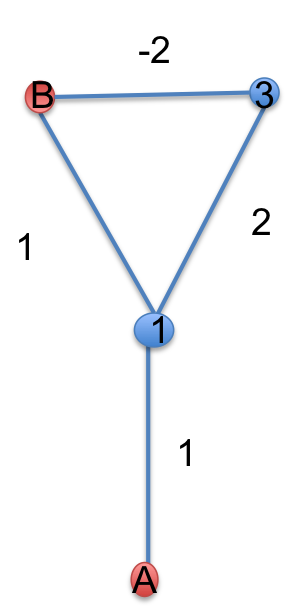
\includegraphics[width=0.20\textwidth]{images/fig1}
		\end{center}
		Note that the minimum distance path from $A$ to $B$ is $1$
		(through edges of cost $1$, $2$ , $-2$) but
		Dijkstra's algorithm will not find this solution. This is because, after
		expanding the only vertex attached to $A$ we will then choose the
		minimum distance vertex, $B$ . Once at
		$B$ the search terminates with a final path length of $2$.
		\item 
		The following figure shows the first three steps of an execution of Dijkstra's
		algorithm to find a path from $A$ to $B$. On the last step the
		distance value of the green vertex changes.
		\begin{center}
		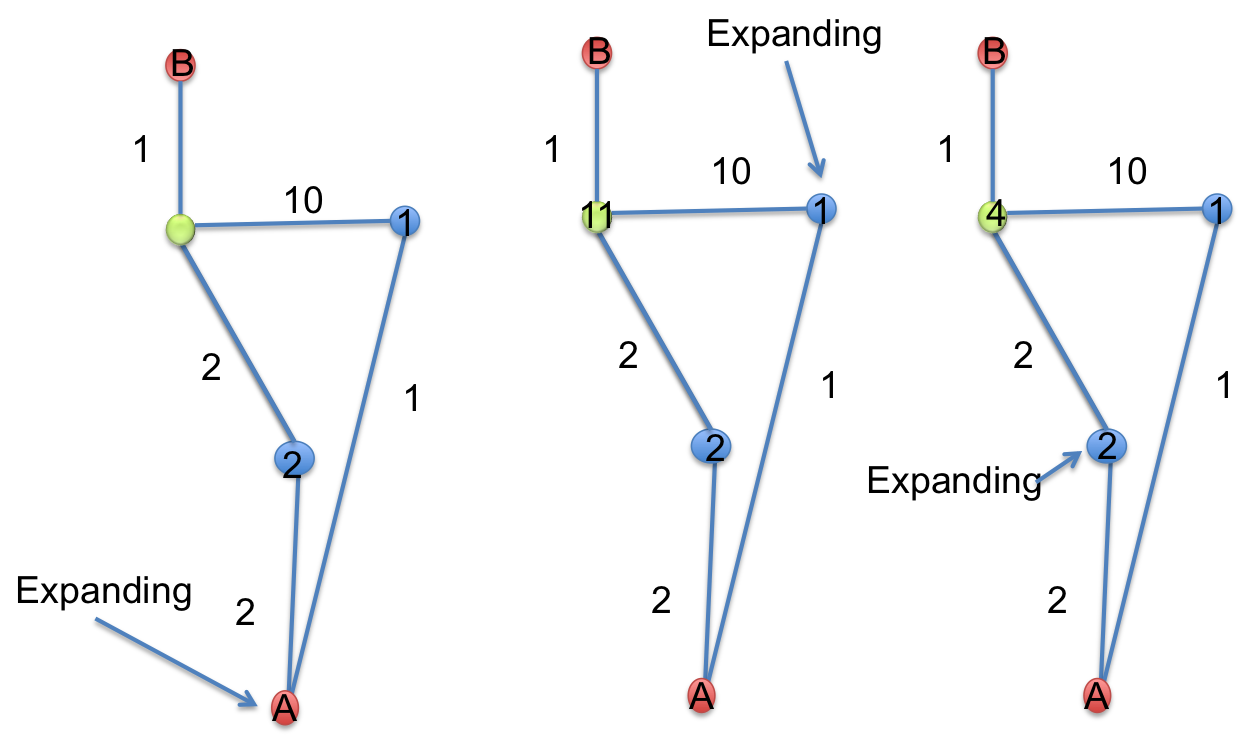
\includegraphics[width=0.80\textwidth]{images/fig2}
		\end{center}
		\item
			\begin{enumerate}
			\item Let $V = \{v_1, v_2 ... v_n \}$.
			To connect all $n$
				vertices $E = \{(v_1,v_2),(v_2,v_3), ... ,
				(v_{n-1},v_n) \}$. So $|E| = n - 1$.
			\item Let $V = \{v_1, v_2 ... v_n \}$.
			 The maximum set of edges for an undirected graph with
					no parallel edges or cycles is 
					$$ E = \{ (v_i,v_j) | i < j \}  $$
					To see why this is,
				first consider a fully connected graph and
				notice how the requirement that our graph lacks
					parallel edges means we have to remove 
					edges of the form $(v_i,v_i)$. And the
					requirement that we lack 
				cycles means we have to remove either
					all edges $(v_i,v_j)$ such that
					$i > j$,
					or all edges such that $i < j$,
					As these connect back to previously
					connected components.\\
					We can see that
				           $$ |E| = \sum_{i=1}^ni = \frac{n(n-1)}{2} $$
                        \item
				To do this we will use a hash set to keep track of
                                        nodes we've already seen, call
                                        it \textit{seen}, start a counter $i$ at
                                        $i = 0$ and run it till $i = n$.
                                        Our algorithm is as follows.
                        \begin{itemize}
                                \item Check node $v_i$ is in
                                        \textit{seen} (constant time). If it is
                                        increment $i$ by one and repeat this
                                        step if it isn't continue.
                                \item Increment the number of connected
                                        components by one.
                                \item If node $v_i$ is \textit{seen}, advance to
                                        the next step, otherwise
                                        recurse \footnote{You could accomplish
                                        this without recursion by using the
                                        doubly linked list to backtrack instead.
                                        This would probably be a little faster
                                        but its on the same runtime and more
                                        difficult to describe.} to all
                                        nodes with an edge to  $v_i$ and apply
                                        this step on them. Then add  $v_i$ to
                                        \textit{seen}.
                                \item Increment $i$ by one and return to the
                                        top.
                        \end{itemize}
                                        Continue this process until $i = n$.
                                        We can see that once we increment our
                                        counter of components we recursively
                                        add
                                        every node in the components
                                        to our seen table. In this way we ensure that
                                        whenever we come across an unseen node
                                        it belongs to a new component.\\
                                        The runtime of the first step is $O(n)$
                                        the runtime of the $3$rd step is
                                        $O(n+m)$ as for all $n$ initially unseen nodes it
                                        will need to recurse through all of
                                        there edges. Our runtime is
                                        $$ O(n) + O(n+m) = O(n+m)$$	
			
			\end{enumerate}
		\item 
		\textbf{Algorithm}
		Use Dijkstra's algorithm by first constructing a
		graph where $V$ is the set of paths and $E$ the set of edges
			connecting every location $(i,j)$ with $(i+1,j)
		(i-1,j), (i,j+1)$ and $(i,j-1)$. We can see that construction of this
		graph runs in linear time. From here we will consider the
		highest of the two points, the end point (reporting the path
		backwards at the end if need be), and set the
		costs on the edges to $0$ for any positive elevation
		change, or the absolute value of the elevation change,
	if the change is negative. From there we can run Dijkstra's algorithm
		on the graph and report the minimum cost path.\\
		\textbf{Correctness}
		The idea here is we want to use Dijkstra's algorithm to find 
                most efficient path. To do this we must first consider
                what an inefficient move is.\\
		Again we will swap the start and end points so that the path goes
		uphill.
                Let $V = \{v_1,v_2,...,v_n\}$ be the vertices of our path and
                let $e(v_i)$ be the elevation at $v_i$. We can see that $f$ the
                amount of fuel used along our path is
		$$f = \sum_{i=2}^n  \max(0,e(v_{i}) - e(v_{i-1})) $$
                and 
		$$\sum_{i=2}^n  e(v_{i}) - e(v_{i-1}) = e(v_n) - e(v_1) $$
                Which is constant regardless of the path taken between $v_1$ and
                $v_n$.
                So inefficiency along any path comes from making moves that
                decrease in elevation. That is
                moves from $v_i$ to $v_{i+1}$ such that $e(v_i) <
                e(v_{i+1})$. Put another way, going downhill is inefficient
		because we know we will have to make up any elevation we lose
		later on. So we assign a cost to these moves equal to how
		inefficient they are, $e(v_{i+1}) - e(v_{i})$.
                \footnote{We could also define the least inefficient
                path as the path with the smallest number of positive
                elevation changes and make negative elevation changes have a cost of
                zero. We would still find the correct solution eventually and
                the runtime would still be the same if the map
                were finite. However we would first check every square that went
                down in elevation so we would probably spend a lot of time
                descending and
                looking for paths near the base of the mountain and only
                reluctantly start climbing it once we are out of other
                options.}\\
                From here correctness from Dijkstra's algorithm ensure that we
                will eventually find the most efficient path.\\
		\textbf{Runtime}
                The runtime here is simply the runtime of Dijkstra's
                algorithm, plus the linear time construction of the graph.
                $$O(m + n\log{n}) + O(n) = O(m + n\log{n})$$.\\
		\item 
		\textbf{Algorithm}
		As we did above, create a start vertex with zero cost edges to
		every element of $S_0$. Here we will manufacture
		multiple end vertices for every $S_i$ and run Dijkstra's algorithm
		until we find all of them (reporting every path without our
		constructed start and end vertices every time we find one).\\
		\textbf{Correctness} 
		Correctness of every individual path follows from correctness of
		the previous answer. \\
		\textbf{Runtime}
		Note: in the worst case scenario Dijkstra's algorithm visits every
		vertex in the graph, so adding multiple endpoints won't impact
		the runtime as, excluding any overhead from reporting, the runtime
		to find all endpoints will be the same as the runtime to find
		only the farthest endpoint from $S_0$.
		\item  
		\textbf{Algorithm} Starting with a vertex $t \in V$. We've run
		Dijkstra's algorithm so we know $d[t]$ that is the total
		cost of the path from $s$ to $t$. Let $x$ be the node before $t$
		on this path. We can see that if $c_x$ is the edge cost between $x$
		and $t$
		$$d[t] = d[x] + c_x$$
		So all we have to do is check nodes connected to $x$ until we
		find a node that meets that condition. If there are two that do
		so, either one will work. Continue backtracking in this
		way till you get to $s$. Record the nodes you pass as you do so
		then print them in reverse order for a path $s \rightarrow t$.\\
		\textbf{Correctness}
		 We let Dijkstra's algorithm fully execute, so for every node $v$
		 $d[v]$ is the distance of the shortest path. Also note that there
		 will be at least one node $x$ such that $d[t] = d[x] + c_x$ and
		 if
		$d[t] < d[x] + c_x$  then $\delta(s,t) <  \delta(s,x) +
		\delta(x,t)$ implying $x$ is not a vertex on the minimum path.
		By induction we can conclude that
		the elements we return represent the shortest path from $x$ to
		$t$.\\
		\textbf{Runtime}
		We can assume that checking all vertices connected to a particular
		vertex takes constant time, and we must do this for every node
		in the minimum path. Call the number of nodes in the minimum
		path $k$. Our runtime is 
		$$O(ck) = O(k)$$
		\item 
		\textbf{Algorithm}
		Consider the set of all points to be the tops and bottoms of every
		vertical line. Also maintain $d[v]$ for all points on the grid in the
		same way you would using Dijkstra's algorithm.
		\begin{itemize}
			\item Add $(x_1,y_1)$ to a priority queue with a
				priority of zero.
			\item Pop an element from the priority queue, call it
				$(x_n,y_n)$, 
				and consider every point $(x_m,y_m)$
				such that $x_n < x_m$. If you can draw a
				straight line from $(x_n,y_n)$ to $(x_m,y_m)$,
				without intersecting any of the given vertical
				lines,
				add it to the priority queue with priority equal
				to $d[(x_n,y_n)]$ plus the distance
				between it and $(x_n,y_n)$ (updating
				$d[(x_m,y_m)]$ if need be).  Repeat this step
				until you pop your endpoint from the queue.
			\item Use the method described in question $8$ to
				backtrack and find the shortest path.\\
		\end{itemize}
		Below is an illustration of the first two expansions of the
		algorithm on the sample data with the edge weights written in
		blue and the distance values for each node written in black.
		\begin{center}
		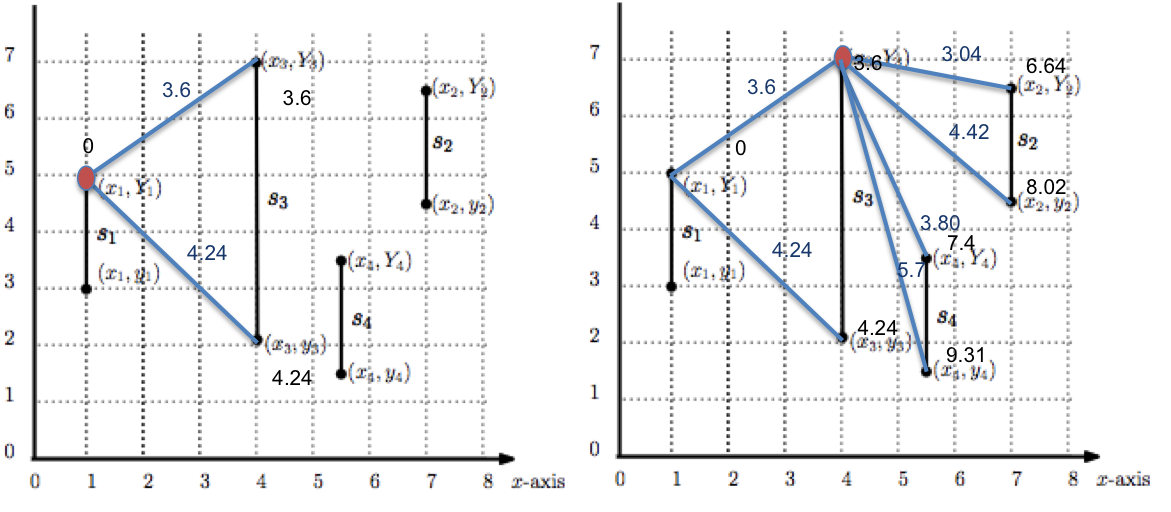
\includegraphics[width=1.00\textwidth]{images/fig3}
		\end{center}
		We can see that the next node to be expanded is $(x_3,y_3)$ as it has
		the lowest $d$ value of any on the grid. Once there are no
		nodes on the fringe with $d$ values above $6.64$ we pop the
		final node from the fringe and are left with the following path.\\
		\begin{center}
		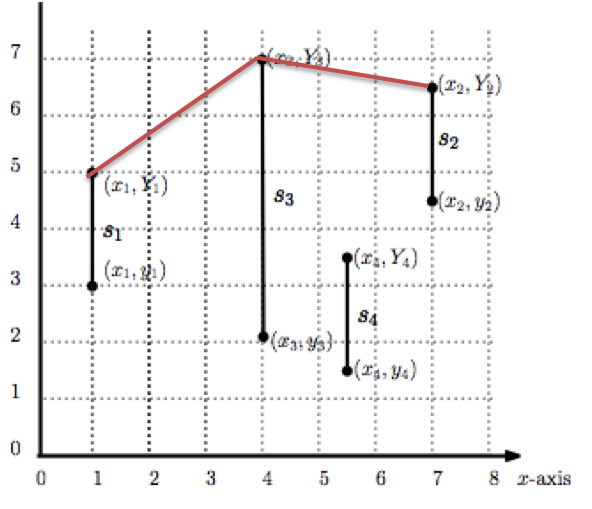
\includegraphics[width=0.55\textwidth]{images/fig4}
		\end{center}
		\textbf{Correctness}
				First note that the shortest possible path
				through the vertical lines will consist of
				straight lines between points on the grid. While
				this makes sense intuitively, 
				proving this rigorously would be difficult. However, the
				main idea here is induction on 
				Euclid's \textit{classic axiom}, the
				shortest path between any two points is a
				line. \\
				Next
				consider a graph with a vertex representing
				every point on the grid, with
				edges representing where there is a straight line between
				the two points that does not intersect any of
				the given lines and a weight equal to the
				length of that line. Observe that the
				minimum cost path through this graph will
				correspond to the minimum distance path through
				the grid. Note that for every path
				between your start and end points consisting of
				straight 
				lines between points on your grid there will be a
				path through your graph representing it. Once
				again the proof of correctness for Dijkstra's
				algorithm implies that this algorithm will find
				the shortest path on the graph/grid.\\
		\textbf{Runtime}
			For every point you consider you will have to look at
			every other point on the grid with a greater $x$
			coordinate, and for all of those points you will have to
			check to see if the line you draw in between them
			intersects with any given vertical, to
			make sure you can draw a straight line between them.
			Because there will be $O(n)$ points of greater $x$
			coordinates for
			any point and $O(n)$ vertical lines to check for
			intersection of the line drawn between the two points
			  the runtime of our algorithm is
			$$nO(n)O(n) = O(n^3)$$
\end{enumerate}
\end{document}
